% Options for packages loaded elsewhere
\PassOptionsToPackage{unicode}{hyperref}
\PassOptionsToPackage{hyphens}{url}
\PassOptionsToPackage{dvipsnames,svgnames,x11names}{xcolor}
%
\documentclass[
  12pt,
  letterpaper,
  DIV=11,
  numbers=noendperiod]{scrreprt}

\usepackage{amsmath,amssymb}
\usepackage{iftex}
\ifPDFTeX
  \usepackage[T1]{fontenc}
  \usepackage[utf8]{inputenc}
  \usepackage{textcomp} % provide euro and other symbols
\else % if luatex or xetex
  \usepackage{unicode-math}
  \defaultfontfeatures{Scale=MatchLowercase}
  \defaultfontfeatures[\rmfamily]{Ligatures=TeX,Scale=1}
\fi
\usepackage{lmodern}
\ifPDFTeX\else  
    % xetex/luatex font selection
\fi
% Use upquote if available, for straight quotes in verbatim environments
\IfFileExists{upquote.sty}{\usepackage{upquote}}{}
\IfFileExists{microtype.sty}{% use microtype if available
  \usepackage[]{microtype}
  \UseMicrotypeSet[protrusion]{basicmath} % disable protrusion for tt fonts
}{}
\usepackage{xcolor}
\setlength{\emergencystretch}{3em} % prevent overfull lines
\setcounter{secnumdepth}{5}
% Make \paragraph and \subparagraph free-standing
\ifx\paragraph\undefined\else
  \let\oldparagraph\paragraph
  \renewcommand{\paragraph}[1]{\oldparagraph{#1}\mbox{}}
\fi
\ifx\subparagraph\undefined\else
  \let\oldsubparagraph\subparagraph
  \renewcommand{\subparagraph}[1]{\oldsubparagraph{#1}\mbox{}}
\fi


\providecommand{\tightlist}{%
  \setlength{\itemsep}{0pt}\setlength{\parskip}{0pt}}\usepackage{longtable,booktabs,array}
\usepackage{calc} % for calculating minipage widths
% Correct order of tables after \paragraph or \subparagraph
\usepackage{etoolbox}
\makeatletter
\patchcmd\longtable{\par}{\if@noskipsec\mbox{}\fi\par}{}{}
\makeatother
% Allow footnotes in longtable head/foot
\IfFileExists{footnotehyper.sty}{\usepackage{footnotehyper}}{\usepackage{footnote}}
\makesavenoteenv{longtable}
\usepackage{graphicx}
\makeatletter
\def\maxwidth{\ifdim\Gin@nat@width>\linewidth\linewidth\else\Gin@nat@width\fi}
\def\maxheight{\ifdim\Gin@nat@height>\textheight\textheight\else\Gin@nat@height\fi}
\makeatother
% Scale images if necessary, so that they will not overflow the page
% margins by default, and it is still possible to overwrite the defaults
% using explicit options in \includegraphics[width, height, ...]{}
\setkeys{Gin}{width=\maxwidth,height=\maxheight,keepaspectratio}
% Set default figure placement to htbp
\makeatletter
\def\fps@figure{htbp}
\makeatother
% definitions for citeproc citations
\NewDocumentCommand\citeproctext{}{}
\NewDocumentCommand\citeproc{mm}{%
  \begingroup\def\citeproctext{#2}\cite{#1}\endgroup}
\makeatletter
 % allow citations to break across lines
 \let\@cite@ofmt\@firstofone
 % avoid brackets around text for \cite:
 \def\@biblabel#1{}
 \def\@cite#1#2{{#1\if@tempswa , #2\fi}}
\makeatother
\newlength{\cslhangindent}
\setlength{\cslhangindent}{1.5em}
\newlength{\csllabelwidth}
\setlength{\csllabelwidth}{3em}
\newenvironment{CSLReferences}[2] % #1 hanging-indent, #2 entry-spacing
 {\begin{list}{}{%
  \setlength{\itemindent}{0pt}
  \setlength{\leftmargin}{0pt}
  \setlength{\parsep}{0pt}
  % turn on hanging indent if param 1 is 1
  \ifodd #1
   \setlength{\leftmargin}{\cslhangindent}
   \setlength{\itemindent}{-1\cslhangindent}
  \fi
  % set entry spacing
  \setlength{\itemsep}{#2\baselineskip}}}
 {\end{list}}
\usepackage{calc}
\newcommand{\CSLBlock}[1]{\hfill\break\parbox[t]{\linewidth}{\strut\ignorespaces#1\strut}}
\newcommand{\CSLLeftMargin}[1]{\parbox[t]{\csllabelwidth}{\strut#1\strut}}
\newcommand{\CSLRightInline}[1]{\parbox[t]{\linewidth - \csllabelwidth}{\strut#1\strut}}
\newcommand{\CSLIndent}[1]{\hspace{\cslhangindent}#1}

\usepackage{pdflscape}
\newcommand{\blandscape}{\begin{landscape}}
\newcommand{\elandscape}{\end{landscape}}
\KOMAoption{captions}{tableheading}
\makeatletter
\@ifpackageloaded{float}{}{\usepackage{float}}
\floatstyle{plain}
\@ifundefined{c@chapter}{\newfloat{algo}{h}{loalgo}}{\newfloat{algo}{h}{loalgo}[chapter]}
\floatname{algo}{Algoritmo}
\newcommand*\listofalgos{\listof{algo}{List of Algoritmos}}
\makeatother
\makeatletter
\@ifpackageloaded{caption}{}{\usepackage{caption}}
\AtBeginDocument{%
\ifdefined\contentsname
  \renewcommand*\contentsname{Índice}
\else
  \newcommand\contentsname{Índice}
\fi
\ifdefined\listfigurename
  \renewcommand*\listfigurename{Lista de Figuras}
\else
  \newcommand\listfigurename{Lista de Figuras}
\fi
\ifdefined\listtablename
  \renewcommand*\listtablename{Lista de Tabelas}
\else
  \newcommand\listtablename{Lista de Tabelas}
\fi
\ifdefined\figurename
  \renewcommand*\figurename{Figura}
\else
  \newcommand\figurename{Figura}
\fi
\ifdefined\tablename
  \renewcommand*\tablename{Tabela}
\else
  \newcommand\tablename{Tabela}
\fi
}
\@ifpackageloaded{float}{}{\usepackage{float}}
\floatstyle{ruled}
\@ifundefined{c@chapter}{\newfloat{codelisting}{h}{lop}}{\newfloat{codelisting}{h}{lop}[chapter]}
\floatname{codelisting}{Listagem}
\newcommand*\listoflistings{\listof{codelisting}{Lista de Listagens}}
\makeatother
\makeatletter
\makeatother
\makeatletter
\@ifpackageloaded{caption}{}{\usepackage{caption}}
\@ifpackageloaded{subcaption}{}{\usepackage{subcaption}}
\makeatother
\makeatletter
\@ifpackageloaded{algorithm}{}{\usepackage{algorithm}}
\makeatother
\makeatletter
\@ifpackageloaded{algpseudocode}{}{\usepackage{algpseudocode}}
\makeatother
\makeatletter
\@ifpackageloaded{caption}{}{\usepackage{caption}}
\makeatother
\ifLuaTeX
\usepackage[bidi=basic]{babel}
\else
\usepackage[bidi=default]{babel}
\fi
\babelprovide[main,import]{brazilian}
% get rid of language-specific shorthands (see #6817):
\let\LanguageShortHands\languageshorthands
\def\languageshorthands#1{}
\ifLuaTeX
  \usepackage{selnolig}  % disable illegal ligatures
\fi
\usepackage{bookmark}

\IfFileExists{xurl.sty}{\usepackage{xurl}}{} % add URL line breaks if available
\urlstyle{same} % disable monospaced font for URLs
\hypersetup{
  pdfauthor={Gabriel de Jesus Pereira},
  pdflang={pt-br},
  colorlinks=true,
  linkcolor={blue},
  filecolor={Maroon},
  citecolor={Blue},
  urlcolor={Goldenrod},
  pdfcreator={LaTeX via pandoc}}

\title{
\includegraphics[width=1in,height=\textheight]{includes/ufpb.png}

Escrever título (escolher no final)}
\usepackage{etoolbox}
\makeatletter
\providecommand{\subtitle}[1]{% add subtitle to \maketitle
  \apptocmd{\@title}{\par {\large #1 \par}}{}{}
}
\makeatother
\subtitle{Universidade Federal da Paraíba - CCEN}
\author{Gabriel de Jesus Pereira}
\date{9 de setembro de 2024}

\begin{document}
\maketitle

\numberwithin{algorithm}{chapter}
\algrenewcommand{\algorithmiccomment}[1]{\hskip3em$\rightarrow$ #1}

\floatname{algorithm}{Algoritmo}

\renewcommand*\contentsname{Índice}
{
\hypersetup{linkcolor=}
\setcounter{tocdepth}{2}
\tableofcontents
}
\renewcommand{\listalgorithmname}{Lista de algoritmos}
\bgroup
\hypersetup{linkcolor = black}
\listofalgorithms
\egroup

\bgroup
\hypersetup{linkcolor = black}
\listoffigures
\egroup

\chapter{Resumo}\label{resumo}

\chapter{Introdução}\label{introduuxe7uxe3o}

\section{Objetivos}\label{objetivos}

\subsection{Objetivo Geral}\label{objetivo-geral}

\subsection{Objetivos Específicos}\label{objetivos-especuxedficos}

\section{Organização do Trabalho}\label{organizauxe7uxe3o-do-trabalho}

\newpage

\chapter{Recursos Computacionais}\label{recursos-computacionais}

\subsection{Linguagem de Programação
R}\label{linguagem-de-programauxe7uxe3o-r}

\subsection{Linguagem de Programação
Python}\label{linguagem-de-programauxe7uxe3o-python}

\subsection{Quarto}\label{quarto}

\subsection{Linguagem de Programação
Python}\label{linguagem-de-programauxe7uxe3o-python-1}

\subsection{Web Scraping}\label{web-scraping}

\newpage

\chapter{Algoritmos de Aprendizado de
Máquina}\label{algoritmos-de-aprendizado-de-muxe1quina}

~~~Neste capítulo, serão descritos os algoritmos de aprendizado de
máquina utilizados neste trabalho. Alguns dos métodos utilizados podem
fazer uso de diversos algoritmos ou modelos estatísticos. No entanto, o
foco principal e o mais utilizado foram as árvores de decisão,
especialmente em sua forma particular, as árvores de regressão. Assim,
os algoritmos descritos são métodos baseados em árvores.

\vspace{12pt}

~~~Os métodos baseados em árvore envolvem a estratificação ou
segmentação do espaço dos preditores\footnote{O espaço dos preditores é
  o conjunto de todos os valores possíveis para as variáveis
  independentes \(\mathbf{x}\)} em várias regiões simples. Dessa forma,
todos os algoritmos utilizados neste trabalho partem dessa ideia.
Portanto, o primeiro a ser explicado será o de árvores de decisão, pois
fundamenta todos os outros algoritmos. Depois das árvores de decisão,
serão explicados os métodos ensemble e, por fim, diferentes variações do
método de gradient boosting.

\section{Árvores de decisão}\label{uxe1rvores-de-decisuxe3o}

~~~Árvores de decisão podem ser utilizadas tanto para regressão quanto
para classificação. Elas servem de base para os modelos baseados em
árvores empregados neste trabalho, focando particularmente nas árvores
de regressão\footnote{Uma árvore de regressão é um caso específico da
  árvore de decisão, mas para regressão.}. O processo de construção de
uma árvore se baseia no particionamento recursivo do espaço dos
preditores, onde cada particionamento é chamado de nó e o resultado
final é chamado de folha ou nó terminal. Em cada nó, é definida uma
condição e, caso essa condição seja satisfeita, o resultado será uma das
folhas desse nó. Caso contrário, o processo segue para o próximo nó e
verifica a próxima condição, podendo gerar uma folha ou outro nó. Veja
um exemplo na Figura~\ref{fig-arvore}.

\begin{figure}

\centering{

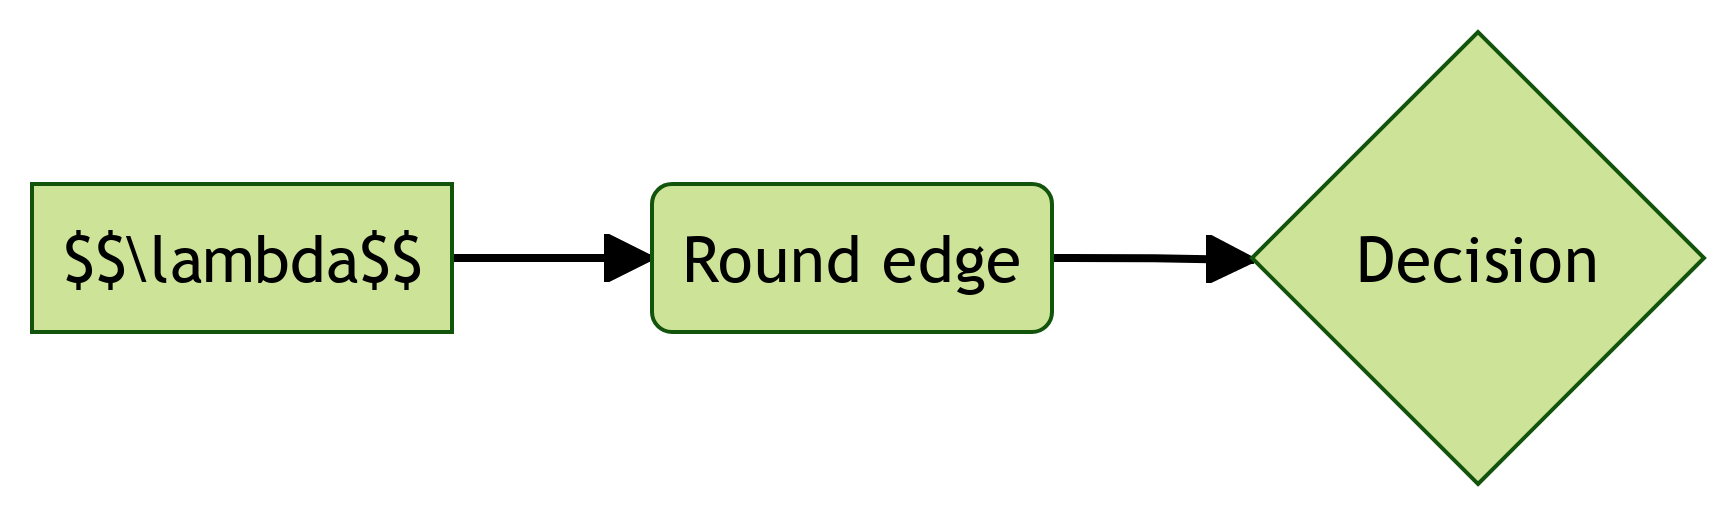
\includegraphics[width=5.5in,height=3.4in]{TCC_files/figure-latex/mermaid-figure-1.png}

}

\caption{\label{fig-arvore}Exemplo de estrutura de árvore de regressão.
A árvore tem cinco folhas e quatro nós internos.}

\end{figure}%

\vspace{12pt}

~~~O espaço dos preditores é dividido em \(J\) regiões distintas e
disjuntas denotadas por \(R_1, R_2, \dots, R_J\). Essas regiões são
construídas em formato de caixa de forma a minimizar a soma dos
quadrados dos resíduos. Dessa forma, pode-se modelar a variável resposta
como uma constante \(c_j\) em cada região \(R_j\)

\[
f\left(x\right) = \sum^J_{j=1}c_j I\left(x \in R_j \right)
\]

~~~O estimador para a constante \(c_j\) é encontrado pelo método de
mínimos quadrados. Assim, deve-se minimizar
\(\sum_{x_i \in R_j} \left[y_i - f\left(x_i\right)\right]^2\). No
entanto, perceba que \(f\left(x_i\right)\) está sendo avaliado somente
em um ponto específico \(x_i\), o que reduzirá \(f\left(x_i\right)\)
para uma constante \(c_j\). É fácil de se chegar ao resultado se for
observada a definição da função indicadora \(I\left(x \in R_j\right)\)

\[
I_{R_j}(x_i) =
\begin{cases}
    1,& \text{se } x_i \in R_j \\
    0,& \text{se } x_i \notin R_j
\end{cases}
\] Como as regiões são disjuntas, \(x_i\) não pode estar simultaneamente
em duas regiões. Assim, para um ponto específico \(x_i\), apenas um dos
casos da função indicadora será diferente de 0. Portanto,
\(f\left(x_i\right) = c_j\). Agora, derivando
\(\sum_{x_i \in R_j}\left(yi - c_j\right)^2\) em relação a \(c_j\)

\begin{equation}\phantomsection\label{eq-partialdev}{
\frac{\partial}{\partial{c_j}}\sum_{x_i \in R_j} \left(y_i - c_j\right)^2 = -2\sum_{x_i \in R_j} \left(y_i - c_j\right)
}\end{equation} e igualando Equação~\ref{eq-partialdev} a 0, tem-se a
seguinte igualdade

\[
\sum_{x_i \in R_j} \left(y_i - \hat{c}_j\right) = 0
\] que se abrirmos o somatório e dividirmos pelo número total de pontos
\(N_j\) na região \(R_j\), teremos que o estimador de \(c_j\) será
simplesmente a média dos \(y_i\) na região \(R_j\):

\begin{equation}\phantomsection\label{eq-estimacjdev}{
\sum_{x_i \in R_j} y_i - \hat{c}_j N_j = 0 \Rightarrow \hat{c}_j = \frac{1}{N_{j}}\sum_{x_i \in R_j} y_i
}\end{equation}

\vspace{12pt}

No entanto, JAMES \emph{et al.} (2013) caracteriza como inviável
considerar todas as possíveis partições do espaço das variáveis em \(J\)
caixas devido ao alto custo computacional. Dessa forma, a abordagem a
ser adotada é uma divisão binária recursiva. O processo começa no topo
da árvore de regressão, o ponto em que contém todas as observações, e
continua sucessivamente dividindo o espaço dos preditores. As divisões
são indicadas como dois novos ramos na árvore, como pode ser visto na
Figura~\ref{fig-arvore}.

\vspace{12pt}

Para executar a divisão binária recursiva, deve-se primeiramente
selecionar a variável independente \(X_j\) e o ponto de corte \(s\) tal
que a divisão do espaço dos preditores conduza a maior redução possível
na soma dos quadrados dos resíduos. Dessa forma, definimos dois
semi-planos

\[
R_{1}\left(j, s\right) = \{X | X_j \leq s\} \text{ e } R_{2}\left(j, s\right) = \{X | X_j > s\}
\] e procuramos a divisão da variável \(j\) e o ponto de corte \(s\) que
resolve a equação

\[
\min_{j, s}\left[\min_{c_1} \sum_{x_i \in R_1\left(j, s\right)} \left(y_i - c_{1}\right)^2 + \min_{c_2} \sum_{x_i \in R_2\left(j, s\right)} \left(y_i - c_{2}\right)^2\right]
\] em que \(c_1\) e \(c_2\) é a média da variável dependente para as
observações de treinamento nas regiões \(R_1\left(j, s\right)\) e
\(R_2\left(j, s\right)\), respectivamente. Assim, encontrando a melhor
divisão, os dados são particionados nas duas regiões resultantes e o
processo de divisão é repetido em todas as outras regiões.

\vspace{12pt}

~~~O tamanho da árvore pode ser considerado um hiperparâmetro para
regular a complexidade do modelo, pois uma árvore muito grande pode
causar sobreajuste aos dados de treinamento, capturando não apenas os
padrões relevantes, mas também o ruído. Como resultado, o modelo pode
apresentar bom desempenho nos dados de treinamento, mas falhar ao lidar
com novos dados devido à sua incapacidade de generalização. Por outro
lado, uma árvore muito pequena pode não captar padrões, relações e
estruturas importantes presentes nos dados. Dessa forma, a estratégia
adotada para selecionar o tamanho da árvore consiste em crescer uma
grande árvore \(T_0\), interrompendo o processo de divisão apenas ao
atingir um tamanho mínimo de nós. Posteriormente, a árvore \(T_0\) é
podada utilizando o critério de custo complexidade, que será definido a
seguir.

\vspace{12pt}

~~~Para o processo de poda da árvore, definimos uma árvore qualquer
\(T\) que pode ser obtida através do processo da poda de \(T_0\), de
modo que \(T \subset T_0\). Assim, sendo \(N_j\) a quantidade de pontos
na região \(R_j\), seja

\[
Q_j\left(T\right) = \frac{1}{N_j} \sum_{x_i \in R_j}\left(y_i - \hat{c}_j\right)^2
\] uma medida de impureza do nó pelo erro quadrático médio. Assim,
define-se o critério de custo complexidade

\[
C_{\alpha}\left(T\right) = \sum_{m = 1}^{|T|}N_jQ_j\left(T\right) + \alpha |T|
\] onde \(|T|\) denota a quantidade total de folhas, e \(\alpha \geq 0\)
é um hiperparâmetro que equilibra o tamanho da árvore e a adequação aos
dados. A ideia é encontrar, para cada \(\alpha\), a árvore
\(T_{\alpha} \subset T_0\) que minimiza \(C_{\alpha}\left(T\right)\).
Valores grandes de \(\alpha\) resultam em árvores menores, enquanto
valores menores resultam em árvores maiores, e \(\alpha = 0\) resulta na
própria árvore \(T_0\). A busca por \(T_{\alpha}\) envolve colapsar
sucessivamente o nó interno que provoca o menor aumento em
\(\sum_j N_j Q_j\left(T\right)\), continuando o processo até produzir
uma árvore com um único nó. Esse processo gera uma sequência de
subárvores, na qual existe uma única subárvore menor que, para cada
\(\alpha\), minimiza \(C_{\alpha}\left(T\right)\).

\vspace{12pt}

~~~A estimação de \(\alpha\) é realizada por validação cruzada com cinco
ou dez folds, sendo \(\hat \alpha\) escolhido para minimizar a soma dos
quadrados dos resíduos durante o processo de validação cruzada. Assim, a
árvore final será \(T_{\hat \alpha}\). O
 Algoritmo~\ref{algo-buildtree}  exemplifica o processo de crescimento
de uma árvore de regressão:

\begin{algo}

\centering{

\begin{algorithm}[H]
\caption{Algoritmo para crescer uma árvore de regressão}
\begin{algorithmic}
\State \textbf{1.} Use a divisão binária recursiva para crescer uma árvore grande $T_0$ nos dados de treinamento, parando apenas quando cada folha tiver menos do que um número mínimo de observações.

\vspace{3.7pt}

\State \textbf{2.} Aplique o critério custo de complexidade à árvore grande \( T_0 \) para obter uma sequência de melhores subárvores \( T_\alpha \), em função de \( \alpha \).

\vspace{3.7pt}

\State \textbf{3.} Use validação cruzada $K\text{-fold}$ para escolher \( \alpha \). Isto é, divida as observações de treinamento em $K$ folds. Para cada \( k = 1, \ldots, K \):
    \State \hspace{1em} (a) Repita os Passos 1 e 2 em todos os folds, exceto no $k\text{-ésimo}$ fold dos dados de
    \State \hspace{1em} treinamento.
    \State \hspace{1em} (b) Avalie o erro quadrático médio de previsão nos dados no $k\text{-ésimo}$ fold deixado
    \State \hspace{1em} de fora, em função de \( \alpha \). Faça a média dos resultados para cada valor de \( \alpha \) e
    \State \hspace{1em} escolha \( \alpha \) que minimize o erro médio.

\vspace{3.7pt}

\State \textbf{4.} Retorne a subárvore \( T_{\hat{\alpha}} \) do Passo 2 que corresponde ao valor estimado de \( \alpha \).
\end{algorithmic}
\end{algorithm}

}

\caption{\label{algo-buildtree}Fonte: JAMES \emph{et al.} (2013, p.
337).}

\end{algo}%

\vspace{12pt}

~~~No caso de uma árvore de decisão para classificação, a principal
diferença está no critério de divisão dos nós e na poda da árvore. Para
a classificação, a previsão em um nó \(j\), correspondente a uma região
\(R_j\) com \(N_j\) observações, será simplesmente a classe majoritária.
Assim, tem-se

\[
\hat{p}_{jk} = \frac{1}{N_j}\sum_{x_i \in R_j} I\left(y_i = k\right)
\] como a proporção de observações da classe \(k\) no nó \(j\). Dessa
forma, as observações no nó \(j\) são classificadas na classe
\(k\left(j\right) = \arg \max_{k} \hat{p}_{jk}\), que é a moda no nó
\(j\).

\vspace{12pt}

~~~Para a divisão dos nós no caso da regressão, foi utilizado o erro
quadrático médio como medida de impureza. Para a classificação, algumas
medidas comuns para \(Q_j\left(T\right)\) são o erro de classificação, o
índice de Gini ou a entropia cruzada.

\section{Métodos Ensemble}\label{muxe9todos-ensemble}

~~~As árvores de decisão são conhecidas por sua alta interpretabilidade,
mas geralmente apresentam um desempenho preditivo inferior em comparação
com outros modelos e algoritmos. No entanto, é possível superar essa
limitação construindo um modelo preditivo que combina a força de uma
coleção de estimadores base, um processo conhecido como aprendizado em
conjunto (Ensemble Learning). De acordo com HASTIE \emph{et al.} (2009),
o aprendizado em conjunto pode ser dividido em duas etapas principais: a
primeira etapa consiste em desenvolver uma população de algoritmos de
aprendizado base a partir dos dados de treinamento, e a segunda etapa
envolve a combinação desses algoritmos para formar um estimador
agregado. Portanto, nesta seção, serão definidos os métodos de
aprendizado em conjunto utilizados neste trabalho.

\subsection{Bagging}\label{bagging}

~~~O algoritmo de Bootstrap Aggregation, ou Bagging, foi introduzido por
BREIMAN (1996). Sua ideia principal é gerar um estimador agregado a
partir de múltiplas versões de um preditor, que são criadas por meio de
amostras bootstrap do conjunto de treinamento, utilizadas como novos
conjuntos de treinamento. O Bagging pode ser empregado para melhorar a
estabilidade e a precisão de modelos ou algoritmos de aprendizado de
máquina, além de reduzir a variância e evitar o sobreajuste. Por
exemplo, o Bagging pode ser utilizado para melhorar o desempenho da
árvore de regressão descrita anteriormente.

\vspace{12pt}

~~~BREIMAN (1996) define formalmente o algoritmo de Bagging, que utiliza
um conjunto de treinamento \(\mathcal{L}\). A partir desse conjunto, são
geradas amostras bootstrap \(\mathcal{L}^{(B)}\) com \(B\) réplicas,
formando uma coleção de modelos \(\{f(x, \mathcal{L}^{(B)})\}\), onde
\(f\) representa um modelo estatístico ou algoritmo treinado nas
amostras bootstrap para prever ou classificar uma variável dependente
\(y\) com base em variáveis independentes \(\mathbf{x}\). Se a variável
dependente \(y\) for numérica, a predição é obtida pela média das
previsões dos modelos:

\[
f_{B}\left(x\right) = \frac{1}{B} \sum_{b = 1}^B f \left(x, \mathcal{L}^{\left(B\right)}\right)
\] onde \(f_{B}\) representa a predição agregada. No caso em que \(y\)
prediz uma classe, utiliza-se a votação majoritária. Ou seja, se
estivermos classificando em classes \(j \in {1, \dots, J}\), então
\(N_j = \#\{B; f(x, \mathcal{L}^{(b)}) = j\}\) representa o número de
vezes que a classe \(j\) foi predita pelos estimadores. Assim,

\[
f_{B}\left(x\right) = \arg \max_{j} N_j
\] isto é, o \(j\) para o qual \(N_j\) é máximo

\vspace{12pt}

~~~Embora a técnica de Bagging possa melhorar o desempenho de uma árvore
de regressão ou de classificação, isso geralmente vem ao custo de menor
interpretabilidade. Quando o Bagging é aplicado a uma árvore de
regressão, construímos \(B\) árvores de regressão usando \(B\) réplicas
de amostras bootstrap e tomamos a média das predições resultantes (JAMES
\emph{et al.}, 2013). Nesse processo, as árvores de regressão crescem
até seu máximo, sem passar pelo processo de poda, resultando em cada
árvore individual com alta variância e baixo viés. No entanto, ao
agregar as predições das \(B\) árvores, a variância é reduzida.

\vspace{12pt}

~~~Para mitigar a falta de interpretabilidade do método Bagging aplicado
a árvores de regressão, pode-se usar a medida de impureza baseada no
erro quadrático médio, definida anteriormente, como uma métrica de
importância das variáveis independentes. Um valor elevado na redução
total média do erro quadrático médio, calculado com base nas divisões
realizadas por um determinado preditor em todas as \(B\) árvores, indica
que o preditor é importante.

\vspace{12pt}

~~~As árvores construídas pelo algoritmo de árvore de decisão se
beneficiam da proposta de agregação do Bagging, mas esse benefício é
limitado devido à correlação positiva existente entre as árvores. Se as
árvores forem variáveis aleatórias independentes e identicamente
distribuídas, cada uma com variância \(\sigma^2\), a variância da média
das previsões das \(B\) árvores será \(\frac{1}{B} \sigma^2\). No
entanto, se as árvores forem apenas identicamente distribuídas, mas não
necessariamente independentes, e apresentarem uma correlação positiva
\(\rho\), a esperança da média das \(B\) árvores será a mesma que a
esperança de uma árvore individual. Portanto, o viés do agregado das
árvores é o mesmo das árvores individuais, e a melhoria é alcançada
apenas pela redução da variância. A variância da média das previsões
será dada por:

\begin{equation}\phantomsection\label{eq-cor}{
\rho \sigma^2 + \frac{1 - \rho}{B}\sigma^2
}\end{equation}

~~~Isso significa que, à medida que o número de árvores \(B\) aumenta, o
segundo termo da soma se torna menos significativo. Portanto, os
benefícios da agregação proporcionados pelo algoritmo de Bagging são
limitados pela correlação entre as árvores (HASTIE \emph{et al.}, 2009).
Mesmo com o aumento do número de árvores no Bagging, a correlação entre
elas impede que as previsões individuais sejam completamente
independentes, resultando em menor diminuição da variância da média das
previsões do que seria esperado se as árvores fossem totalmente
independentes. Uma maneira de melhorar o algoritmo de Bagging é por meio
do Random Forest, que será descrito a seguir.

\subsection{Random Forest}\label{random-forest}

~~~O algoritmo Random Forest é uma técnica derivada do método de
Bagging, mas com modificações específicas na construção das árvores. O
objetivo é melhorar a redução da variância ao diminuir a correlação
entre as árvores, sem aumentar significativamente a variabilidade. Isso
é alcançado durante o processo de crescimento das árvores por meio da
seleção aleatória de variáveis independentes.

\begin{algo}

\centering{

\begin{algorithm}[H]
\caption{Algoritmo de uma Random Forest para regressão ou classificação}
\begin{algorithmic}
\State \hspace{1em} \textbf{1.} Para b = 1 até B:

\vspace{0.8em}

    \State \hspace{2em} (a) Construa amostras bootstrap $\mathbf{\mathcal{L}}^*$ de tamanho \( N \) dos dados de
    \State \hspace{2em} \vspace{0.1em} treinamento.

    \State \hspace{2em} (b) Faça crescer uma árvore de floresta aleatória \( T_b \) para os dados bootstrap,
    \State \hspace{2em} repetindo recursivamente os seguintes passos para cada folha da árvore, até que
    \State \hspace{2em} \vspace{0.5em} o tamanho mínimo do nó \( n_{min} \) seja atingido.
    \State \hspace{4em} \vspace{0.1em} i. Selecione \( m \) variáveis aleatoriamente entre as \( p \) variáveis.
    \State \hspace{4em} \vspace{0.1em} ii. Escolha a melhor variável entre as \( m \).
    \State \hspace{4em} \vspace{0.1em} iii. Divida o nó em dois subnós.

\vspace{0.8em}

\State \hspace{1em} \textbf{2.} Por fim, o conjunto de árvores \( \{T_b\}^{B}_1\) é construído.

\vspace{1em}

\State \hspace{0.7em} No caso da regressão, para fazer uma predição em um novo ponto \( x \), temos a seguinte função:


$$
\hat{f}^{B}_{rf}\left(x\right) = \frac{1}{B}\sum^{B}_{b = 1} T_{b}\left(x\right)
$$

\vspace{1em}

\State \hspace{0.7em} Para a classificação é utilizado o voto majoritário. Assim, seja $\hat{C}_{b}\left(x\right)$ a previsão da classe da árvore de floresta aleatória $b$. Então,

$$
\hat{C}^{B}_{rf}\left(x\right) = \arg \max_c \sum^{B}_{b = 1}I\left(\hat{C}_b\left(x\right) = c\right)
$$

\State onde $c$ representa as classes possíveis.

\end{algorithmic}
\end{algorithm}

}

\caption{\label{algo-rf}Fonte: HASTIE \emph{et al.} (2009, p. 588).}

\end{algo}%

\vspace{12pt}

~~~ No algoritmo Random Forest, ao construir uma árvore a partir de
amostras bootstrap, antes de cada divisão, selecionam-se aleatoriamente
\(m \leq p\) das \(p\) variáveis independentes como candidatas para a
divisão (com \(m = p\) no caso do Bagging). Apenas uma dessas \(m\)
variáveis é usada para realizar a divisão, com base em critérios como a
minimização da impureza. Diferentemente do Bagging, que tende a gerar
árvores de decisão semelhantes e, portanto, previsões altamente
correlacionadas, o Random Forest visa minimizar esse problema ao
proporcionar oportunidades para que outros preditores sejam
considerados. Assim, em média, \(\left(p - m\right)/p\) das divisões nem
sequer considerarão o preditor mais forte, permitindo que outros
preditores também tenham a chance de serem usados (JAMES \emph{et al.},
2013). Esse processo de redução da correlação entre as árvores resulta
em uma média das árvores menos variável e, consequentemente, mais
confiável.

\vspace{12pt}

~~~A quantidade de variáveis independentes \(m\) selecionadas
aleatoriamente é um hiperparâmetro que pode ser estimado por meio de
validação cruzada. Valores comuns para \(m\) são
\(m=\sqrt{p}\)\hspace{0pt} com tamanho mínimo do nó igual a um para
classificação, e \(m=p/3\)\hspace{0pt} com tamanho mínimo do nó igual a
cinco para regressão (HASTIE \emph{et al.}, 2009). Quando o número de
variáveis é grande, mas poucas são realmente relevantes, o algoritmo
Random Forest pode ter um desempenho inferior com valores pequenos de
\(m\), pois isso reduz as chances de selecionar as variáveis mais
importantes. No entanto, usar um valor pequeno de \(m\) pode ser
vantajoso quando há muitos preditores correlacionados. Além disso, assim
como no Bagging, a Random Forest não sofre de sobreajuste com o aumento
da quantidade de árvores \(B\). Portanto, é suficiente usar um \(B\)
grande o bastante para que a taxa de erro se estabilize (JAMES \emph{et
al.}, 2013).

\subsection{Boosting Trees}\label{boosting-trees}

~~~O Boosting, assim como o Bagging, é um método destinado a melhorar o
desempenho de modelos ou algoritmos. No entanto, neste trabalho, o
Boosting foi aplicado apenas às árvores de regressão. Portanto, a
explicação do Boosting será restrito ao caso de Boosting Trees
( Algoritmo~\ref{algo-boos} ).

\vspace{12pt}

\begin{algo}

\centering{

\begin{algorithm}[H]
\caption{Método Boosting aplicado a árvores de regressão}
\begin{algorithmic}
\State \hspace{1em} \textbf{1.} Defina $\hat{f}\left(x\right) = 0 \text{ e } r_i = y_i$ para todos os $i$ no conjunto de treinamento

\vspace{0.8em}

\State \hspace{1em} \vspace{0.8em} \textbf{2.} Para $b = 1, 2, \dots, B$, repita:

  \State \hspace{2em} (a) Ajuste uma árvore $\hat{f}^b$ com $d$ divisões para os dados de
  \State \hspace{2em} \vspace{0.1em} treinamento $\left(X, r\right)$.

  \State \hspace{2em} (b) Atualize $\hat{f}$ adicionando uma versão com o hiperparâmetro $\lambda$ de taxa de
  \State \hspace{2em} aprendizado:

$$
\hat{f}\left(x\right) \gets \hat{f}\left(x\right) + \lambda \hat{f}^b\left(x\right)
$$

  \vspace{0.1em}

  \State \hspace{2em} (c) Atualize os resíduos,

$$
r_i \gets r_i - \lambda \hat{f}^b\left(x_{i}\right)
$$

\vspace{1em}

\State \hspace{1em} \textbf{3.} Retorne o modelo de boosting,

$$
\hat{f}\left(x\right) = \sum_{b = 1}^B \lambda \hat{f}^b\left(x\right)
$$


\end{algorithmic}
\end{algorithm}

}

\caption{\label{algo-boos}Fonte: JAMES \emph{et al.} (2013, p. 349).}

\end{algo}%

~~~No algoritmo de Bagging, cada árvore é construída e ajustada
utilizando amostras bootstrap, e ao final, um estimador agregado
\(\varphi_B\)\hspace{0pt} é formado a partir das \(B\) árvores. O
Boosting Trees funciona de maneira semelhante, mas sem o uso de amostras
bootstrap. A ideia principal é corrigir os erros das árvores anteriores,
ajustando as novas árvores aos resíduos das anteriores, visando melhorar
suas previsões. Assim, as árvores são construídas de forma sequencial,
incorporando as informações das árvores anteriores.

\vspace{12pt}

~~~No caso da regressão, o Boosting combina um grande número de árvores
de decisão \(\hat{f}^1, \dots, \hat{f}^B\). A primeira árvore é
construída utilizando o conjunto de dados original, e seus resíduos são
calculados. Com a primeira árvore ajustada, a segunda árvore é ajustada
aos da árvore anterior resíduos e, em seguida, é adicionada ao estimador
para atualizar os resíduos. Dessa forma, os resíduos servem como
informação crucial para construir novas árvores e corrigir os erros das
árvores anteriores. Como cada nova árvore depende das árvores já
construídas, árvores menores são suficientes (JAMES \emph{et al.},
2013).

\vspace{12pt}

~~~O processo de aprendizado no método de Boosting é lenta, o que acaba
gerando melhores resultados. Esse processo de aprendizado pode ser
controlado por um hiperparâmetro \(\lambda\) chamado de shrinkage, ou
taxa de aprendizado, permitindo que mais árvores, com formas diferentes,
corrijam os erros das árvores passadas. No entanto, um valor muito
pequeno para \(\lambda\) requer uma quantidade muito maior \(B\) de
árvores e, diferente do Bagging e Random Forest, o Boosting pode sofrer
de sobreajuste se a quantidade de árvores é muito grande. Além disso, a
quantidade de divisões \(d\) em cada árvore, que controla a complexidade
do boosting, pode ser considerado também um hiperparâmetro. Para
\(d = 1\) é ajustado um modelo aditivo, já que cada termo involve apenas
uma variável. JAMES \emph{et al.} (2013) define \(d\) como a
profundidade de interação que controla a ondem de interação do modelo
boosting, já que \(d\) divisões podem envolver no máximo \(d\)
variáveis.

\subsection{Stacked generalization}\label{stacked-generalization}

~~~A Stacked Generalization, ou Stacking, é um método de ensemble que
consiste em treinar um modelo gerado a partir da combinação da predição
de vários outros modelos, visando melhorar a precisão das predições.
Esse método pode ser aplicado a qualquer modelo estatístico ou algoritmo
de aprendizado de máquina. A ideia principal é atribuir pesos às
predições, de modo a dar maior importância aos modelos que produzem
melhores resultados, ao mesmo tempo em que se evita atribuir altos pesos
a modelos com alta complexidade.

\vspace{12pt}

~~~Matematicamente, o Stacking define predições
\(\hat{f}_m^{-i}\left(x\right)\) em x, utilizando o modelo \(m\),
aplicado ao conjunto de treinamento com a \(i\text{-ésima}\) observação
removida (HASTIE \emph{et al.}, 2009). Assim, os peso são estimados de
forma a minimizar o erro de predição combinado, dado pela seguinte
expressão:

\[
\hat{w}^{st} = \arg \min_{w} \sum^{N}_{i = 1} \left[y_i - \sum^{M}_{m = 1} w_m f^{-i}_m\left(x_i\right)\right]^2
\] A previsão final dos modelos empilhados é
\(\sum_{m} \hat{w}_m^{st} \hat{f}_m\left(x\right)\). Assim, em vez de
escolher um único modelo, o método de Stacking combina os modelos
utilizando pesos estimados, o que melhora a performance preditiva, mas
pode comprometer a interpretabilidade.

\subsection{Gradient Boosting}\label{gradient-boosting}

~~~O algoritmo de Gradient Boosting é semelhante ao de Boosting, mas com
diferenças mínimas. Ele constrói modelos aditivos ajustando
sequencialmente funções bases aos pseudos-resíduos, que correspondem aos
gradientes da função perda do modelo atual (FRIEDMAN, 2002). Esses
gradientes indicam a direção na qual a função perda diminui. Neste
trabalho, foram utilizadas diferentes implementações de Gradient
Boosting. No entanto, todas empregam o Gradient Boosting com árvores de
regressão, com algumas modificações para a construção das árvores ou
para melhorar a eficiência do algoritmo existente. Assim, o algoritmo a
ser explicado será o Gradient Tree Boosting
( Algoritmo~\ref{algo-gradboos} ).

\begin{algo}

\centering{

\begin{algorithm}[H]
\caption{Gradient Tree Boosting}
\begin{algorithmic}
\State \hspace{1em} \textbf{1.} Inicialize $f_0\left(x\right) = \arg \min_{\gamma} \sum_{i = 1}^N L\left(y_i, \gamma \right)$

\vspace{0.8em}

\State \hspace{1em} \vspace{0.8em} \textbf{2.} Para $m = 1$ até $M$:

  \State \hspace{2em} (a) Para $i = 1, 2, \dots, N$, calcule

$$
{r}_{im} = -\left[\frac{\partial L\left(y_i, f\left(x_i \right)\right)}{\partial f\left(x_i\right)}\right]_{f = f_{m - 1}}
$$

  \State \hspace{2em} (b) Ajuste uma árvore de regressão aos pseudo-resíduos $r_{im}$, obtendo regiões
  \State \hspace{2em} terminais $R_{jm}, \ j = 1, 2, \dots, J$.


  \State \vspace{0.1em}

  \State \hspace{2em} (c) Para $j = 1, 2, \dots, J_m$, calcule

$$
\gamma_{jm} = \arg \min_{\gamma} \sum_{x_i \in R_{jm}} L\left(y_i, f_{m - 1}\left(x_i\right) + \gamma\right)
$$

  \vspace{0.1em}

  \State \hspace{2em} (d) Atualize $f_m\left(x\right) = f_{m - 1}\left(x\right) + \lambda \sum^{J}_{j = 1} \gamma_{jm} I\left(x \in R_{jm}\right)$

\vspace{1em}

\State \hspace{1em} \textbf{3.} Retorne $\hat{f}\left(x\right) = f_M\left(x\right)$

\end{algorithmic}
\end{algorithm}

}

\caption{\label{algo-gradboos}Fonte: HASTIE \emph{et al.} (2009, p.
361).}

\end{algo}%

\vspace{12pt}

O Gradient Boosting aplicado para árvores de regressão, tem que cada
função base é uma árvore de regressão com \(J_m\) folhas. Dessa forma,
cada árvore de regressão tem a forma aditiva

\begin{equation}\phantomsection\label{eq-treebost}{
h_m\left(x;\{b_j, R_j\}^J_{1}\right) = \sum^{J_m}_{j = 1} b_{jm} I\left(x \in R_{jm}\right)
}\end{equation} em que \(\{R_{jm}\}^{J_m}_{1}\) são as regiões disjuntas
que, coletivamente, cobrem o espaço de todos os valores conjuntos das
variáveis preditoras \(\mathbf{x}\). Essas regiões são representadas
pelas folhas de sua correspondente árvore. Como as regiões são
disjuntas, Equação~\ref{eq-treebost} se reduz simplesmente a
\(h_m\left(x\right) = b_{jm}\text{ para } x \in  R_{jm}\). Por mínimos
quadrados, \(b_{jm}\) é simplesmente a média dos pseudo-resíduos
\(r_{im}\),

\[
\hat{b}_{jm} = \frac{1}{N_{jm}} \sum_{x_i \in R_{jm}} r_{im}
\] que dão a direção de diminuição da função perda \(L\) pela expressão
do gradiente da linha 2(a). Assim, cada árvore de regressão é ajustada
aos \(r_{im}\) de forma a minimizar o erro das árvores anteriores.
\(N_{jm}\) denota a quantidade de pontos na região \(R_{jm}\). Por fim,
o estimador é separadamente atualizado em cada região correspondente e é
expresso

\[
f_m\left(x\right) = f_{m - 1}\left(x\right) + \lambda \sum^{J}_{j = 1} \gamma_{jm} I\left(x \in R_{jm}\right)
\] em que \(\gamma_{jm}\) representa a atualização da constante ótima
para cada região, baseado na função perda \(L\), dada a aproximação
\(f_{m-1}\left(x\right)\). O \(0 < \lambda \leq 1\), assim como no
algoritmo de boosting, representa o hiperparâmetro shrinkage para
controlar a taxa de aprendizado. Pequenos valores de \(\lambda\)
necessitam maiores quantidades de iterações \(M\) para diminuir o risco
de treinamento.

\subsection{Diferentes implementações de Gradient
Boosting}\label{diferentes-implementauxe7uxf5es-de-gradient-boosting}

\subsubsection{Light Gradient Boosting}\label{light-gradient-boosting}

\subsubsection{Extreme Gradient
Boosting}\label{extreme-gradient-boosting}

\vspace{12pt}

\chapter{Metodologia}\label{metodologia}

\section{Os dados e o procedimento adotado para sua
obtenção}\label{os-dados-e-o-procedimento-adotado-para-sua-obtenuxe7uxe3o}

--- AINDA SERÁ MODIFICADO ---

~~~O Web scraping, também conhecido como extração de dados da web, é uma
técnica utilizada para o processo de coleta de dados estruturados da web
de maneira automatizada. É um processo que vem sendo constantemente
utilizado por instituições públicas e privadas para a construção de
produtos que utilizam algoritmos de aprendizagem de máquinas, observa
ofertas e discontos, faz análise de mercado ou monitoração de marcas.

\vspace{12pt}

Neste projeto, para fins de estudo e análise do mercado imobiliário, os
dados foram coletados por meio de extração de dados do site do Zap
Imóveis. O Zap Imóveis é um site do Grupo OLX que reúne ofertas do
mercado imobiliário e que funciona como uma plataforma dinâmica para
facilitar a conexão entre quem deseja alugar, comprar ou vender um
imóvel; podendo servir também para corretores ou outros profissionais do
setor de imóveis. Este projeto foi possível graças as informações que
foram coletadas do site do Zap Imóveis em dois diferentes períodos do
ano de 2023. O primeiro deles, as informações foram coletadas utilizando
variados pacotes para raspagem de dados e proxies rotativas da linguagem
de programação R, a fim de evitar ser bloqueado pelos mecanismos de
segurança do site. Na segunda etapa, os dados foram coletados empregando
a linguagem de programação Python com as bibliotecas Scrapy e Playwrite,
que serve para web crawling e web scraping, e o Playwrite que serve para
testes em aplicativos da web, mas que neste caso foi utilizado para
manejar páginas dinâmicas.

\vspace{12pt}

Desta forma, com a ideia de modelar o valor do imóvel e analisar o
mercado imobiliário, foram coletados aqueles variáveis que estavam
disponíveis no site do Zap Imóveis e que poderiam de alguma forma ser
significativas ao tentar explicar o valor do imóvel durante a sua
modelagem. Assim, no total foram coletatas 23 variáveis, das quais 8 são
quantitativas e 15 qualitativas nominais, sendo 13 de caráter
dicotômico. No entanto, nem todas essas variáveis foram coletadas
diretamente do Zap Imóveis, a latitude e longitude foram obtidas pela
geocodificação do endereço utilizando o pacote tidygeocoder da linguagem
de programação R. Portanto, temos as seguites variáveis:

\begin{itemize}
\item
  Valor do imóvel: esta é a variável dependente, aquela que será
  modelada e será o principal objeto de estudo deste trabalho;
\item
  Área: área do imóvel em \(m^2\);
\item
  Condomínio: valor pago pelo condomínio;
\item
  IPTU: imposto cobrado de quem tem um imóvel urbano;
\item
  Banheiro: quantidade de banheiros presentes na propriedade;
\item
  Vaga de estacionamento: quantidade total de vagas de estacionamento;
\item
  Quarto: quantidade de quartos no imóvel;
\item
  Latitude: posição horizontal medida em frações decimais de graus;
\item
  Longitude: posição vertical que, assim como a latitude, é medida em
  frações decimais de graus;
\item
  Tipo do imóvel: foram obtidos 7 tipos de imóveis, apartamentos, casas,
  casas comerciais, casas de condomínio, casas de vila, coberturas,
  lotes comerciais e de condomínio;
\item
  Endereço: nome do endereço do imóvel;
\item
  Variáveis dicotômicas que indicam se o imóvel tem ou não aquela
  característica (representado como 1 ou 0, respectivamente): área de
  serviço, academia, elevador, espaço gourmet, piscina, playground,
  portaria 24 horas, quadra de esporte, salão de festa, sauna, spa e
  varanda gourmet.
\end{itemize}

\vspace{12pt}

No entanto, devido a observações feitas durante o estudo, nem todas
essas variáveis foram utilizadas para a modelagem do valor dos imóveis,
seja por conter muitos valores valores ausentes ou por não ter se
mostrado significante para o que se desejava explicar. Ainda, como a
coleta destes dados foram feitas em dois momentos distintos, temos dois
bancos de dados, um com 29712 observações e o outro com 14956. Por fim,
essas duas bases de dados foram unidas e, para não correr o risco de
conter imóveis repetidos, aqueles que tinham o mesmo número de
identificação foram removidos.

\section{Descritiva dos dados}\label{descritiva-dos-dados}

~~~A análise exploratória de dados marca uma das primeiras etapas de
qualquer estudo que utiliza a estatística como uma de suas principais
ferramentas, pois permite encontrar padrões de comportamento no dados,
descobrir relações entre as variáveis estudadas. Dessa forma, a primeira
etapa desse estudo, após a coleta e organização dos dados obtidos do Zap
Imóveis, foi fazer uma descritiva dos dados. Essa etapa permitiu
encontrar padrões nos diferentes tipos de imóveis bem como o seu tipo
pode influenciar na características do imóvel, o que, por consequência,
pode afetar o seu valor. Assim, para identificar esses diferentes
comportamentos, foram criados gráficos e tabelas a fim de caracterizar
as relações das variáveis independentes com a dependente.

\section{Reamostragem para avaliação de
performance}\label{reamostragem-para-avaliauxe7uxe3o-de-performance}

\section{Métricas de avaliação}\label{muxe9tricas-de-avaliauxe7uxe3o}

\section{Tunagem de
hiperparâmetros}\label{tunagem-de-hiperparuxe2metros}

\vspace{12pt}

\vspace{12pt}

A busca pela melhor combinação de hiperparâmetros \(\lambda\) é feito de
forma iterativa, utilizando métodos de reamostragem para dividir o
conjunto de dados entre teste e treinamento. Portanto, para validar e
encontrar os hiperparâmetos, o algoritmo de aprendizagem é validado
através da divisão do conjunto de dados. Assim, tem-se a seguinte
estratégia de separação do conjunto de dados:

\begin{equation}\phantomsection\label{eq-teste}{
\mathcal{J} = \left(\left(J_{treino, 1},\ J_{teste, 1}\right), ..., \left(J_{treino, B},\ J_{test, B}\right)\right)
}\end{equation} onde \(J_{treino, i}, \ J_{teste, i}\) representam os
vetores de índices \(\left(i = 1, \, 2, ..., \ B\right)\) para os
conjuntos de treino e teste, respectivamente, e \(B\) representa o
número total de divisões.

\vspace{12pt}

A motivação para fazer a divisão do conjunto de dados entre treino e
teste é ajustar o algoritmo em dados reais e avaliar a sua performance
em dados ainda não vistos, processo representado pelo banco de treino e
teste, respectivamente. Para fazer a avaliação dessa performance é
necessário estimar uma métrica de performance em cada divisão. Assim,
para um dado algoritmo \(I_{\lambda}\) é calculado uma métrica de
performance \(\rho\) para cada \(J_{teste, i}\) após o ajuste do
algoritmo no \(J_{treino, i}\). Por fim, pode ser calculado uma média
amostral da métrica de cada uma das divisões. Dessa forma, o problema de
otimizar os hiperparâmetros pode ser definida da seguinte forma:

\[
\lambda^* \in \underset{\lambda \in \tilde \Lambda}{\operatorname{argmin}} \ c\left(\lambda \right)
\] onde \(\lambda^*\) denota a melhor combinação possível de
hiperparâmetros, \(c\left(\lambda \right)\) representa a generalização
do erro, podendo ser representado também por
\(\widehat{GE}\left(I, \ \mathcal J, \ \rho, \ \lambda\right)\), quando
\(I, \ \mathcal{J}, \ \rho\) são fixados e \(I\) denota um algoritmo de
aprendizagem de máquina. O erro de generalização é estimado e otimizado
a fim de evitar um ajuste excessivo (overfitting), podendo prejudicar
quando o algoritmo fizer estimativas em dados ainda não vistos. Assim, o
processo pode ser visualizado pela figura Figura~\ref{fig-hpo}:

\begin{figure}

\centering{

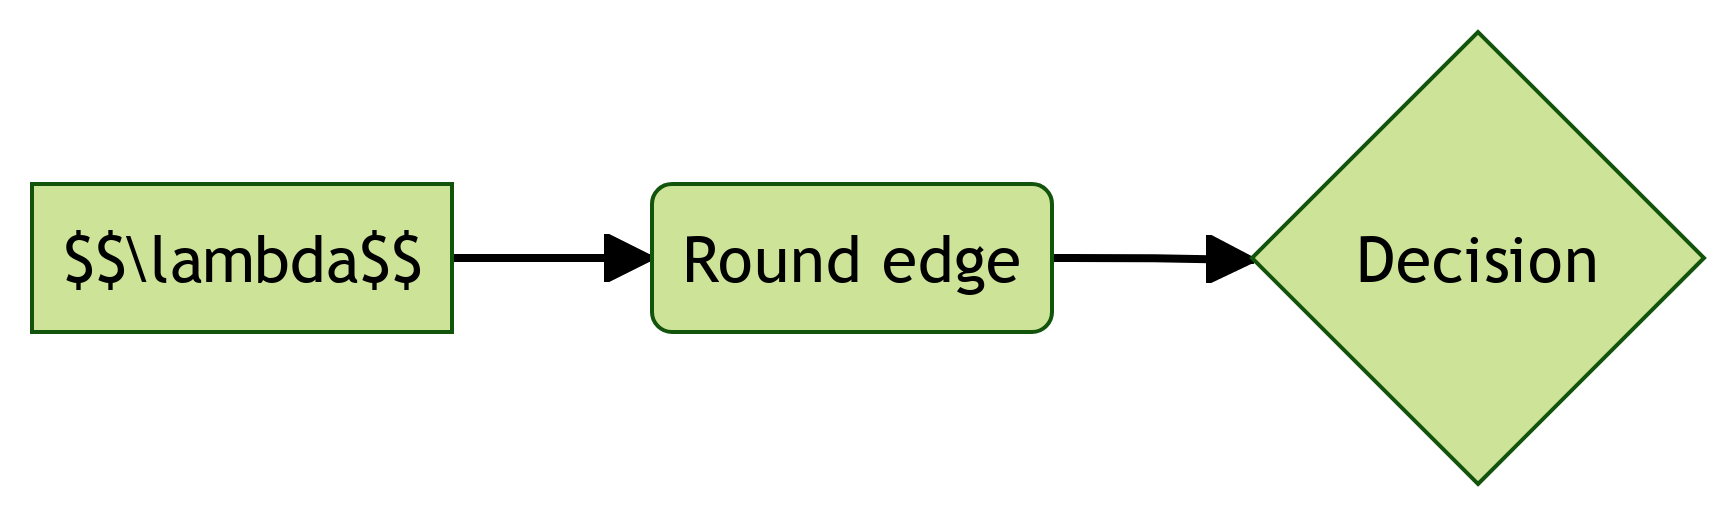
\includegraphics[width=4.5in,height=1.34in]{TCC_files/figure-latex/mermaid-figure-2.png}

}

\caption{\label{fig-hpo}Processo de otimização de hiperparâmetros}

\end{figure}%

\vspace{12pt}

\subsection{Otimização Bayesiana}\label{otimizauxe7uxe3o-bayesiana}

~~~Existem diversas técnicas para otimização de hiperparâmetros
utilizadas em aprendizagem de máquina. Uma das técnicas mais comuns é o
GridSearch. BISCHL \emph{et al.} (2023) definem GridSearch como um
processo que divide o intervalo contínuo de valores possíveis de cada
hiperparâmetro em um conjunto de valores específicos e avalia
exaustivamente o algoritmo para todas as combinações possíveis. No
entanto, como todas as combinações possíveis aumentam exponencialmente
com a quantidade necessária para avaliação do algoritmo, o GridSearh tem
um custo computacional bastante elevado. Assim, existem algoritmos de
otimização mais sofisticados que entregam melhores performances, como a
otimização bayesiana, que foi utilizada neste trabalho.

\vspace{12pt}

~~~A otimização bayesiana não se refere a um tipo específico de
algoritmo de otimização, mas sim a uma filosofia de otimização baseada
em inferência bayesiana, a qual contém uma extensa família de algoritmos
de otimização (GARNETT, 2023). Não obstante, a otimização bayesiana tem
obtido benchmarks melhores que outros algoritmos em inúmeros problemas
complexos de otimização de hiperparâmetros (SNOEK; LAROCHELLE; ADAMS,
2012).

\vspace{12pt}

~~~Diferente de outros algoritmos de otimização de hiperparâmetros, a
otimização bayesiana determina as futuras tentativas de avaliação com
base em resultados obtidos previamente (YANG; SHAMI, 2020). Para a
definição dos pontos futuros, é utilizada uma função probabilística
\(P\left(\rho |  \lambda \right)\) (BERGSTRA; YAMINS; COX, 2013). Assim,
após o ajuste da função probabilística, tem-se como resultado para cada
\(\lambda\) uma estimativa da performance
\(\hat c \left(\lambda \right)\) e da predição da incerteza
\(\hat \sigma \left(\lambda \right)\), além de obter também a
distribuição preditiva da função probabilística. Com a distribuição
obtida, uma função de aquisição determina o trade-off entre exploitation
e exploration\footnote{exploitation pode ser entendido como procurar
  próximo a boas observações e}. Dessa forma, os algoritmos de
otimização bayesiana são definidos segundo a lei
\(\lambda \to c\left(\lambda \right)\) e procuram um equilíbrio entre o
processo de exploitation-exploration para detectar as regiões ótimas
mais prováveis e não perder melhores configurações em áreas ainda não
exploradas.

\subsection{Tree-Structured Parzen
Estimator}\label{tree-structured-parzen-estimator}

~~~Existem diversas funções probabilísticas para uso na otimização
bayesiana, algumas delas é o Processo Gaussiano, Random Forest ou
Tree-Structured Parzen Estimator (TPE). Nesse trabalho, foi utilizado o
Tree-Structured Parzen Estimator, utilizando a biblioteca Optuna (AKIBA
\emph{et al.}, 2019) para sua aplicação.

\vspace{12pt}

~~~O TPE define duas funções,
\(l\left(x\right) \text{ e } g\left(x\right)\), que são usadas para
modelar a distribuição das variáveis do domínio (YANG; SHAMI, 2020).
Utilizando as duas densidades, o TPE procura modelar a probabilidade de
se observar um hiperparâmetro \(x\) dado uma métrica de performance
\(\rho\). Dessa forma, tem-se a seguinte definição:

\begin{equation}\phantomsection\label{eq-tpe}{
p(x|y) =
\begin{cases}
    l(x) & \text{if } y < y^* \\
    g(x) & \text{if } y \ge y^*
\end{cases}
}\end{equation} em que \(l\left(x\right)\) é definido como a densidade
em que a função perda é menor que um limiar \(y^*\) e
\(g\left(x\right)\) representa é a densidade em que a função
perda\footnote{definição de função perda} tem valores acima do limiar
\(y^*\) (BERGSTRA \emph{et al.}, 2011). O limite \(y^*\) é escolhido
através de um hiperparâmetro \(\gamma\), onde \(\gamma\) representa o
percentil dos valores observados de \(y\), de modo que
\(p\left(y < y^*\right) = \gamma\).

\vspace{12pt}

Por padrão, o tree-structured parzen estimator tem como função de
aquisição o Expected Improvement \(\left(EI\right)\), que pode ser
otimizado para o TPE da seguinte forma:

\begin{equation}\phantomsection\label{eq-exp}{
  EI_{y^*}\left(x\right) = \int_{-\infty}^{y^*} \left(y^* - y\right)p\left(y | x\right) dy
}\end{equation}

Ainda, para encontrar a probabilidade marginal de \(x\), temos a
seguinte integral
\(p\left(x\right) = \int_{\mathbb{R}} p\left(x | y\right)p\left(y\right)dy\).
Particionando o domínio de \(y\), chega-se em:

\[
p\left(x\right) = \int_{-\infty}^{y^*} p\left(x | y\right)p\left(y\right)dy + \int_{y^*}^{\infty} p\left(x | y\right)p\left(y\right)dy = \gamma l\left(x\right) + \left(1 - \gamma \right) g\left(x\right)
\]

Assim, utilizando o Teorema de Bayes e fazendo as substituições na
integral da Equação~\ref{eq-exp}:

\[
EI_{y^*}\left(x\right) = \int_{-\infty}^{y^*} \left(y^* - y\right) \frac{p\left(x | y\right)p\left(y\right)}{p\left(x\right)}dy = \left(\gamma y^*  - \int_{-\infty}^{y^*} p\left(y\right)dy\right) \left(\gamma + \left(1 - \gamma\right)\frac{g\left(x\right)}{l\left(x\right)}\right) ^{-1}
\] em que a segunda expressão do produto mostra que para maximizar o
Expected Improvement é necessário pontos de \(x\) com maior
probabilidade em \(l\left(x\right)\) e com baixa probabilidade em
\(g\left(x\right)\). Não obstante, no TPE, maximizar o \(EI\) é
equivalente a maximizar a razão entre as duas distribuições
\(r\left(x\right) = \frac{l\left(x\right)}{g\left(x\right)}\)
(COWEN-RIVERS \emph{et al.}, 2022).

\newpage

\chapter{Resultados}\label{resultados}

\section{Análise exploratória de
dados}\label{anuxe1lise-exploratuxf3ria-de-dados}

~~~A análise exploratória dos dados foi realizada após a divisão entre
os conjuntos de treinamento e teste. Essa abordagem foi adotada para
evitar o sobreajuste do modelo e garantir que o algoritmo não aprenda
com informações indisponíveis no conjunto de teste. Assim, a descritiva
dos dados foi realizada utilizando o conjunto de treinamento.

\vspace{12pt}

~~~A primeira etapa da análise exploratória de dados foi identificar os
dados faltantes e determinar a melhor forma de tratá-los. A
Figura~\ref{fig-miss} mostra a porcentagem de observações ausentes em
cada variável. As variáveis com a maior quantidade de dados ausentes são
o valor do condomínio e o IPTU, pois essas informações são as menos
preenchidas no site de onde os dados foram coletados. A terceira
variável, com quase 20\% de observações ausentes, é a quantidade de
vagas de estacionamento. As variáveis com mais de 20\% de observações
ausentes foram removidas da base de dados, pois, com essa quantidade de
valores faltantes, nem mesmo métodos de imputação proporcionariam um
tratamento adequado. Dessa forma, apenas as variáveis de valor do
condomínio e IPTU foram removidas, enquanto as demais com valores
ausentes foram tratadas por meio de imputação.

\begin{figure}

\centering{

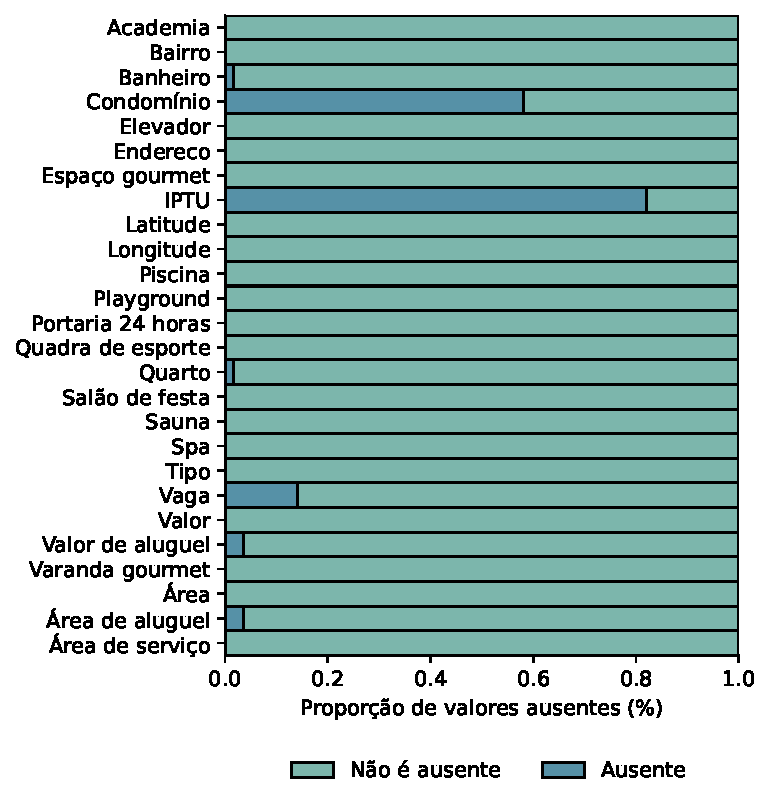
\includegraphics{TCC_files/figure-pdf/fig-miss-output-1.pdf}

}

\caption{\label{fig-miss}Quantidade de valores ausentes por variáveis}

\end{figure}%

\vspace{12pt}

~~~Uma das dificuldades que podem surgir durante a modelagem é o
desbalanceamento das classes, ou seja, a diferença na quantidade de cada
tipo de imóvel. O tipo de imóvel mais predominante no conjunto de dados
são os apartamentos, que representam 81,36\% do total. Em seguida, vêm
as casas, com 8,91\%, e os flats, com 5,72\%. Por fim, as casas
comerciais são as menos representadas, com apenas 15 ocorrências. Esse
desbalanceamento claro entre as classes pode dificultar o desempenho do
modelo, especialmente na previsão de categorias menos frequentes, como
as casas comerciais, onde o modelo pode ter dificuldade em obter bons
resultados.

\vspace{12pt}

~~~A distribuição das variáveis foram análisadas em termos do tipo do
imóvel a partir de um gráfico de violino. Pela Figura~\ref{fig-violin},
é fácil perceber que a maioria das distribuições possuem assimetria
negativa. Os apartamentos possuem caudas longas à direita, indicando
presença de valores extremamente altos e que indicam que talvez seja
necessário a aplicação de alguma transformação para a estabilização da
variância.

\begin{figure}

\centering{

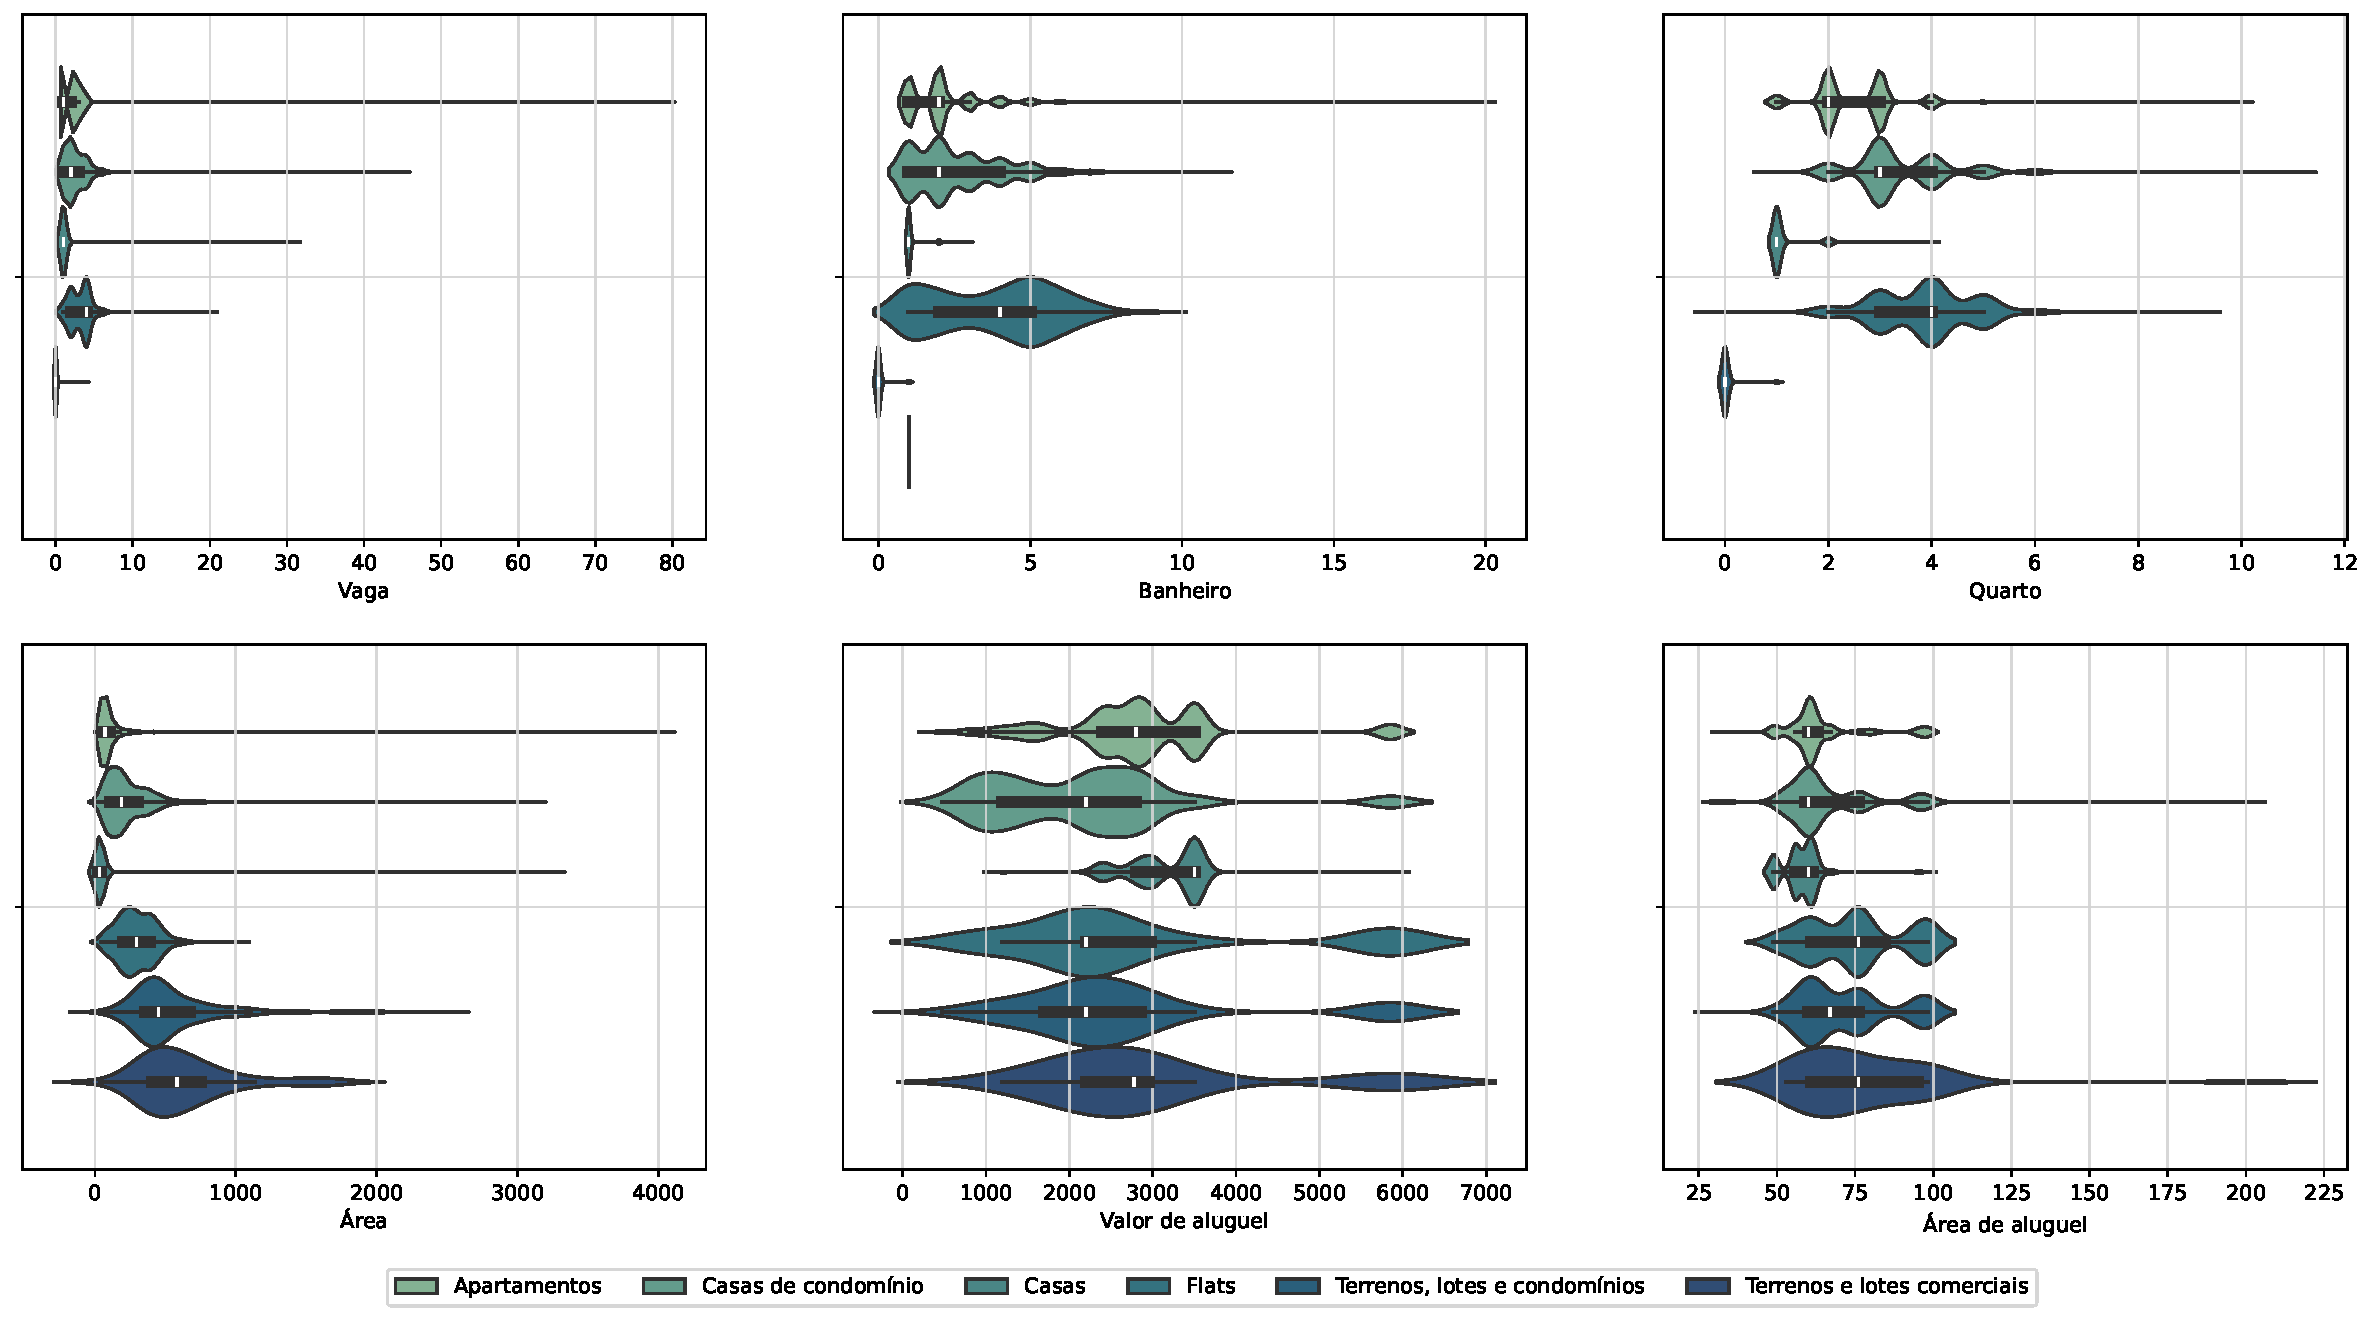
\includegraphics{TCC_files/figure-pdf/fig-violin-output-1.pdf}

}

\caption{\label{fig-violin}Distribuição das variáveis numéricas.}

\end{figure}%

\vspace{12pt}

~~~Para reduzir a assimetria da distribuição dos valores dos imóveis,
foi aplicada uma transformação logarítmica. O gráfico de densidade à
esquerda na Figura~\ref{fig-densitarg} mostra os dados originais da
distribuição do valor dos imóveis. Há uma tendência dos valores ficarem
mais concentrados em uma faixa mais baixa, mas alguns imóveis apresentam
valores excepcionalmente altos, o que acaba gerando uma distribuição
assimétrica positiva. Com a aplicação da transformação logarítmica, a
assimetria é suavizada, comprimindo os valores mais altos. Isso tende a
aproximar a distribuição de uma forma mais simétrica, facilitando a
modelagem e análise estatística.

\begin{figure}

\centering{

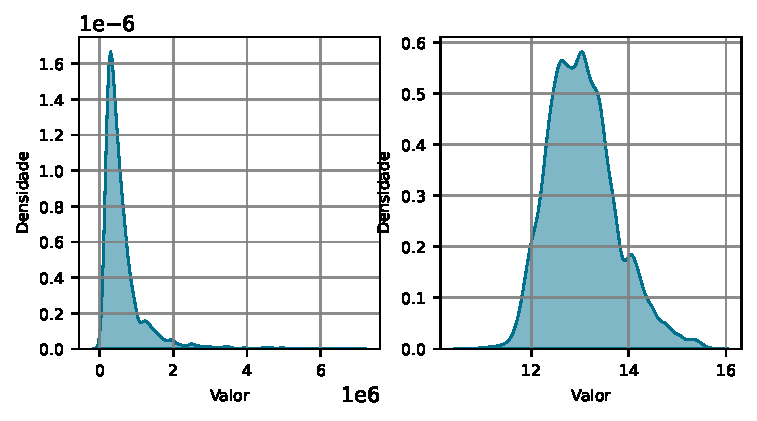
\includegraphics{TCC_files/figure-pdf/fig-densitarg-output-1.pdf}

}

\caption{\label{fig-densitarg}Comparação entre distribuição dos valores
dos imóveis antes e depois da transformação logarítmica.}

\end{figure}%

\vspace{12pt}

~~~A Figura~\ref{fig-corplot} apresenta a matriz de correlação entre as
variáveis numéricas do conjunto de dados. As cores mais escuras indicam
uma correlação mais forte entre as variáveis, enquanto as cores mais
claras indicam o contrário. O valor do imóvel apresenta maior correlação
com as variáveis de área do imóvel e número de vagas de estacionamento.
Além disso, o valor do imóvel tem alta correlação com o valor médio do
aluguel, número de quartos e banheiros, além de ser fortemente
influenciado pela localização das propriedades. Algumas variáveis
apresentam multicolinearidade entre si, mas os algoritmos utilizados
selecionam aleatoriamente as variáveis para a modelagem, o que reduz o
risco de selecionar variáveis redundantes.

\begin{figure}

\centering{

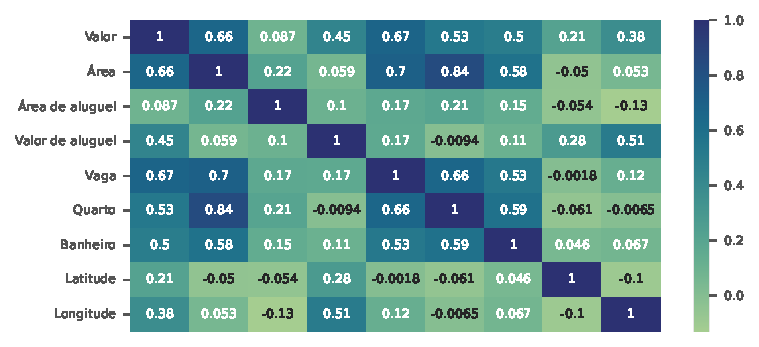
\includegraphics{TCC_files/figure-pdf/fig-corplot-output-1.pdf}

}

\caption{\label{fig-corplot}Gráfico de correlação de Spearman das
variáveis independentes.}

\end{figure}%

\textbf{ADICIONAR NO FIM UM GRÁFICO DE ESPACIALIZAÇÃO DOS DADOS (INCLUIR
VARIAÇÃO DA COR PELO PREÇO DO IMÓVEL)}

\section{Construção dos modelos}\label{construuxe7uxe3o-dos-modelos}

\subsection{Random Forest}\label{random-forest-1}

\subsection{Gradient Boosting}\label{gradient-boosting-1}

\chapter{Conclusão}\label{conclusuxe3o}

\chapter{Referências}\label{referuxeancias}

\phantomsection\label{refs}
\begin{CSLReferences}{0}{1}
\bibitem[\citeproctext]{ref-optuna_2019}
AKIBA, T. \emph{et al.} Optuna: A Next-generation Hyperparameter
Optimization Framework. {[}S.l.{]}: {[}s.n.{]}, 2019.

\bibitem[\citeproctext]{ref-bergstra2011algorithms}
BERGSTRA, J. \emph{et al.} Algorithms for hyper-parameter optimization.
\textbf{Advances in neural information processing systems}, 2011. v. 24.

\bibitem[\citeproctext]{ref-bergstra2013making}
\_\_\_\_\_\_; YAMINS, D.; COX, D. Making a science of model search:
Hyperparameter optimization in hundreds of dimensions for vision
architectures. {[}S.l.{]}: PMLR, 2013. p. 115--123.

\bibitem[\citeproctext]{ref-bischl2023hyperparameter}
BISCHL, B. \emph{et al.} Hyperparameter optimization: Foundations,
algorithms, best practices, and open challenges. \textbf{Wiley
Interdisciplinary Reviews: Data Mining and Knowledge Discovery}, 2023.
v. 13, n. 2, p. e1484.

\bibitem[\citeproctext]{ref-breiman1996bagging}
BREIMAN, L. Bagging predictors. \textbf{Machine learning}, 1996. v. 24,
p. 123--140.

\bibitem[\citeproctext]{ref-cowen2022hebo}
COWEN-RIVERS, A. I. \emph{et al.} Hebo: Pushing the limits of
sample-efficient hyper-parameter optimisation. \textbf{Journal of
Artificial Intelligence Research}, 2022. v. 74, p. 1269--1349.

\bibitem[\citeproctext]{ref-friedman2002stochastic}
FRIEDMAN, J. H. Stochastic gradient boosting. \textbf{Computational
statistics \& data analysis}, 2002. v. 38, n. 4, p. 367--378.

\bibitem[\citeproctext]{ref-garnett2023bayesian}
GARNETT, R. \textbf{Bayesian optimization}. {[}S.l.{]}: Cambridge
University Press, 2023.

\bibitem[\citeproctext]{ref-hastie2009elements}
HASTIE, T. \emph{et al.} \textbf{The elements of statistical learning:
data mining, inference, and prediction}. {[}S.l.{]}: Springer, 2009. V.
2.

\bibitem[\citeproctext]{ref-james2013introduction}
JAMES, G. \emph{et al.} \textbf{An introduction to statistical
learning}. {[}S.l.{]}: Springer, 2013. V. 112.

\bibitem[\citeproctext]{ref-snoek2012practical}
SNOEK, J.; LAROCHELLE, H.; ADAMS, R. P. Practical bayesian optimization
of machine learning algorithms. \textbf{Advances in neural information
processing systems}, 2012. v. 25.

\bibitem[\citeproctext]{ref-yang2020hyperparameter}
YANG, L.; SHAMI, A. On hyperparameter optimization of machine learning
algorithms: Theory and practice. \textbf{Neurocomputing}, 2020. v. 415,
p. 295--316.

\end{CSLReferences}



\end{document}
